\documentclass[conference]{IEEEtran}

\usepackage{cite}
\usepackage{amsmath,amssymb}
\usepackage{graphicx}
\usepackage{xcolor}
\usepackage{booktabs}
\usepackage{array}
\usepackage{multirow}
\usepackage{url}
\usepackage{hyperref}
\hypersetup{colorlinks=false, pdfborder={0 0 0}}

\graphicspath{{figures/}}

\def\BibTeX{{\rm B\kern-.05em{\sc i\kern-.025em b}\kern-.08em
T\kern-.1667em\lower.7ex\hbox{E}\kern-.125emX}}

\begin{document}

\title{An Empirical Evaluation of Large Language Models and Retrieval-Augmented Prompting Strategies for Multi-Language Code Smell Detection}

\author{
\IEEEauthorblockN{Matthew Gregorat}
\IEEEauthorblockA{
\textit{Department of Computer Science} \\
\textit{Florida Polytechnic University} \\
Lakeland, Florida, USA \\
mgregorat0995@floridapoly.edu
}
\and
\IEEEauthorblockN{Erick Orozco}
\IEEEauthorblockA{
\textit{Department of Computer Science} \\
\textit{Florida Polytechnic University} \\
Lakeland, Florida, USA \\
eorozco0824@floridapoly.edu
}
\and
\IEEEauthorblockN{Bibek Gupta}
\IEEEauthorblockA{
\textit{Department of Computer Science} \\
\textit{Florida Polytechnic University} \\
Lakeland, Florida, USA \\
bgupta2957@floridapoly.edu
}
}

\maketitle

\begin{abstract}
Large Language Models (LLMs) are increasingly embedded in developer tooling, yet
their effectiveness at detecting \emph{code smells}, structural anti-patterns that
degrade software maintainability, has not been systematically benchmarked under
controlled prompting conditions across multiple languages. This paper presents an
empirical evaluation of three instruction-tuned LLMs
(\textit{DeepSeek~v3.2~671B}, \textit{Gemma~3~27B-IT}, and \textit{Mistral~Devstral~2~123B})
served through a managed inference endpoint (AWS Bedrock,
\texttt{ap-southeast-2}) on a Fowler-aligned, expert-validated benchmark of
34 annotated files spanning Java, Python, JavaScript, and C++. We design and
compare five prompting strategies, zero-shot, few-shot, taxonomy-tree
chain-of-thought, self-verification, and retrieval-augmented generation
(RAG), and additionally run a \emph{random-retrieval} ablation to isolate the
contribution of retrieval content from the contribution of context length.
Across 18 ($3{\times}6$) configurations on 473 line-level smell labels (21
distinct smells, 5 Fowler categories), we compute pooled micro/macro F1 with
bootstrap confidence intervals and paired-record significance tests. On this
single benchmark the best configuration, \textit{Mistral~Devstral~2~123B}
with dense RAG ($k{=}3$), reaches micro F1 of \textbf{0.964} on the held-out
split, a $+0.272$ absolute lift over zero-shot (95\% CI $[0.191, 0.365]$,
paired bootstrap); we treat this number as a \emph{benchmark-specific} upper
bound, not a population-level accuracy estimate, given the small file count
($n{=}34$) and the absence (in this study) of a contamination probe,
retrieval-leakage check, and multi-seed variance estimates. We find that
few-shot prompting is the single largest and most consistent driver of
accuracy ($+0.161$ mean F1), that taxonomy-tree chain-of-thought and
self-verify prompts \emph{degrade} accuracy on this task, and that dense
retrieval beats random retrieval significantly only for the strongest model.
We release the full evaluation harness, prompts, and per-record predictions
to support reproducibility.
\end{abstract}

\begin{IEEEkeywords}
Large Language Models, Code Smells, Retrieval-Augmented Generation, Empirical
Software Engineering, Prompt Engineering, Static Analysis.
\end{IEEEkeywords}

%======================================================================
\section{Introduction}
%======================================================================

Software maintainability is heavily influenced by the presence of \emph{code
smells}, surface symptoms in source code that are not bugs themselves but indicate
deeper design weaknesses, accelerate technical debt, and inflate long-term
maintenance cost. Traditional static analyzers
(SonarQube, PMD, Checkstyle, SpotBugs) detect smells via fixed rules and metric
thresholds. While fast and deterministic, they are well known to suffer from high
false-positive rates and limited contextual reasoning,
which causes developers to disable or ignore the warnings they emit.

Large Language Models (LLMs) trained on source code have demonstrated strong code
understanding capabilities~\cite{roziere2023codellama}, motivating recent attempts
to apply them to smell detection. However, two gaps remain. First, prior
LLM-for-smell studies typically fix a single prompting strategy, leaving open
the question of \emph{which} prompting recipe (vanilla, in-context examples,
chain-of-thought, self-critique, or retrieval-augmented) actually drives
accuracy on this task. Second, evidence on whether retrieval-augmented
prompting helps detection (as opposed to generation), and whether any such
lift comes from the \emph{content} of retrieved exemplars or simply from the
added context length, is largely missing. We report results for three
instruction-tuned LLMs accessed through a managed inference endpoint
(AWS Bedrock); the underlying model weights are publicly published, but our
measurements characterize the Bedrock-served deployment of those weights
rather than self-hosted inference (see Threats to Validity).

\subsection{Research Questions}
\noindent We investigate three research questions:
\begin{itemize}
 \item \textbf{RQ1.} \textit{Does in-context demonstration (few-shot) improve
 over zero-shot smell detection on instruction-tuned LLMs?}
 \item \textbf{RQ2.} \textit{Does adding explicit reasoning structure, a
 taxonomy tree (P3) or self-verification (P4), improve detection beyond
 zero-shot, or introduce noise?}
 \item \textbf{RQ3.} \textit{Does the \emph{content} of retrieved examples
 matter? Concretely, can dense semantic retrieval ($k{=}3$) outperform a
 random-retrieval control ($k{=}2$) of the same prompt template?}
\end{itemize}

\subsection{Contributions}
This paper makes the following contributions:
\begin{enumerate}
 \item \textbf{A controlled multi-model, multi-prompt benchmark.} We evaluate
 three instruction-tuned LLMs (served through a managed Bedrock endpoint)
 across six prompting conditions on four programming languages, yielding
 72 (model, prompt, language) measurement cells over 473 expert-validated
 smell annotations.
 \item \textbf{A retrieval-content ablation.} We isolate \emph{what} retrieval
 contributes by comparing dense embedding retrieval against a random-retrieval
 placebo holding context length and prompt template constant.
 \item \textbf{Statistically rigorous analysis.} All headline differences are
 accompanied by paired-record bootstrap 95\% confidence intervals on per-file
 micro F1 (1{,}000 resamples, paired by sample\_id), distinguishing real lift
 from sample noise.
 \item \textbf{Actionable findings.} We identify a clear winning configuration
 (Mistral~Devstral~2 + dense RAG, F1$=$0.964), characterize where each model
 fails (long-tail and inheritance smells), and provide practical guidance:
 prefer \emph{few-shot} on smaller models, \emph{add RAG} only on the largest
 model, and avoid taxonomy-tree CoT and self-verification prompts.
 \item \textbf{An open, reproducible harness.} All prompts, datasets,
 predictions, and analysis notebooks are released; every figure in this paper
 is regenerable from a single notebook.
\end{enumerate}

%======================================================================
\section{Background and Related Work}
%======================================================================

\subsection{Code Smells and Fowler's Taxonomy}
Code smells were popularized by Fowler~\cite{fowler2018refactoring} as recurring symptoms of design decay
(e.g., \textit{Long Method}, \textit{Large Class}, \textit{Feature Envy},
\textit{Shotgun Surgery}). They group naturally
into five higher-level categories, \textit{Bloaters},
\textit{Object-Orientation Abusers}, \textit{Change Preventers},
\textit{Dispensables}, and \textit{Couplers}, which we use as auxiliary structure
in our experiments.

\subsection{Rule-Based Static Analyzers}
Industrial tools (SonarQube, PMD, Checkstyle, SpotBugs) flag smells via metric
thresholds (e.g., method length, cyclomatic complexity, parameter count) or
hand-written AST patterns. Their main weakness is contextual blindness: a 200-line
method that is well-decomposed semantically receives the same warning as a 200-line
spaghetti method, leading to documented high false-positive rates in
practice.

\subsection{LLMs for Code Analysis}
Recent work on test smells in LLM-generated
code~\cite{ouedraogo2024test, lucas2024evaluating} shows that LLMs can identify
a meaningful subset of smell-like patterns and confirms that
\emph{prompt design} is at least as influential as model choice. Complementary
benchmarking work has measured the \emph{propensity} of LLMs to themselves
introduce code smells during generation~\cite{velasco2024propense}, underscoring
that smell awareness is a meaningful axis of code-LLM evaluation. Code Llama and
related code-specialized models~\cite{roziere2023codellama} demonstrate that
publicly released model weights can be competitive with commercial APIs on
several code-understanding tasks; the three models we evaluate sit in this
family of publicly published instruction-tuned models served via a managed
inference endpoint.

\subsection{Retrieval-Augmented Generation}
Retrieval-Augmented Generation (RAG)~\cite{lewis2020retrieval} grounds an LLM's
prediction on retrieved context, typically using dense
sentence-embedding similarity~\cite{reimers2019sbert,karpukhin2020dpr}, building on
bidirectional transformer encoders such as BERT~\cite{devlin2019bert}. Prior work has shown
retrieval can improve code generation, but its
value for \emph{detection} (rather than generation) is less clear, particularly
when the target task is already specified by a fixed taxonomy. Crucially, prior
RAG papers rarely separate the \emph{content effect} (relevant examples help)
from the \emph{length effect} (any extra context primes the model). Our random-
retrieval ablation directly addresses this confound.

\subsection{Positioning}
To the best of our knowledge, this is the first study that simultaneously
(i)~evaluates three instruction-tuned LLMs of different families and scales
on a Fowler-aligned multi-language smell benchmark using a single managed
inference endpoint with deterministic decoding,
(ii)~factorially compares five distinct prompting strategies,
(iii)~runs a content-controlled retrieval ablation, and
(iv)~reports paired-bootstrap statistical significance on per-record F1
differences. We position the headline numbers as a benchmark-specific
upper bound for this configuration; we do not claim a population-level
accuracy estimate (see Threats to Validity).

%======================================================================
\section{Dataset Characteristics}
\label{sec:dataset-eda}
%======================================================================

Before reporting model results we summarise the structural properties of
the benchmark. All figures in this section are produced by an EDA
notebook released with the public artifact and are regenerated directly
from the prepared dataset.

\begin{figure}[t]
\centering
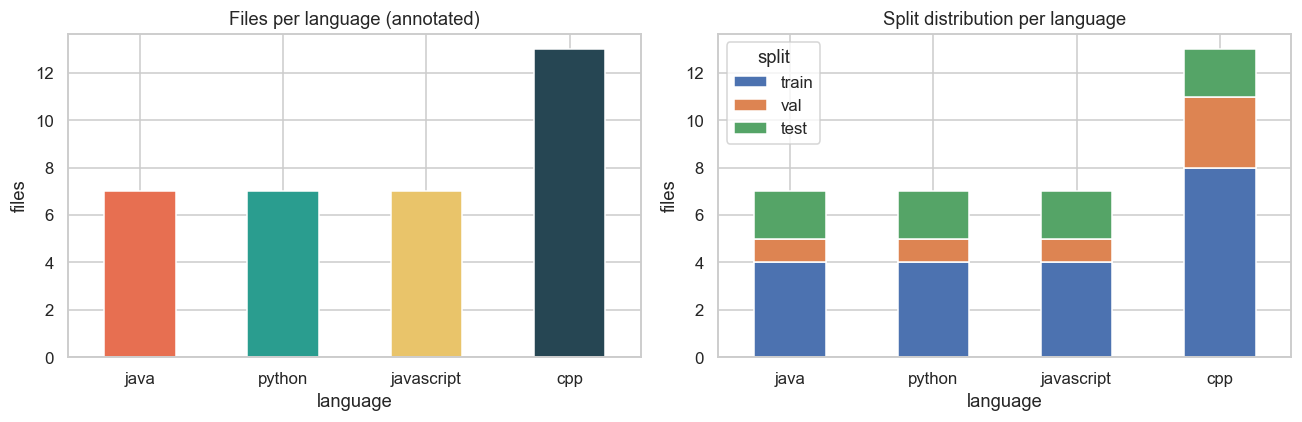
\includegraphics[width=\columnwidth]{01_files_per_language.png}
\caption{Files per language in the harmonised benchmark. C++ has 13
entries because each class ships as paired \texttt{.cpp}/\texttt{.h}
files; Java, Python, and JavaScript each have 7 files.}
\label{fig:eda-files}
\end{figure}

\begin{figure}[t]
\centering
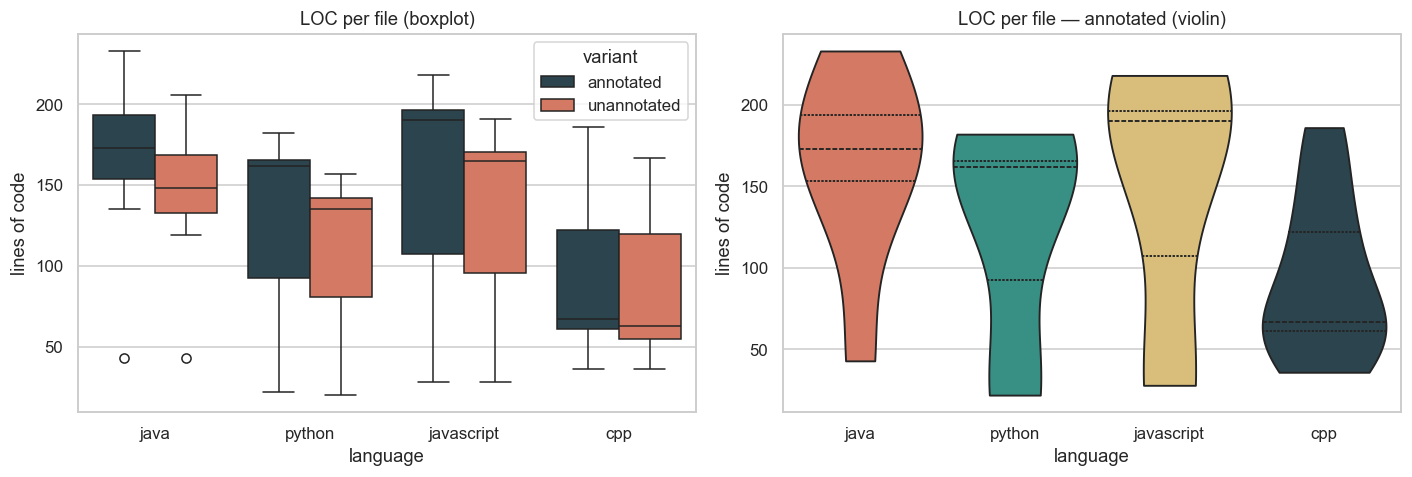
\includegraphics[width=\columnwidth]{02_loc_distribution.png}
\caption{Distribution of lines of code per file. Files are short by
industrial standards (median $\approx$120 LOC), which constrains how
far conclusions generalise to repository-scale code.}
\label{fig:eda-loc}
\end{figure}

\begin{figure}[t]
\centering
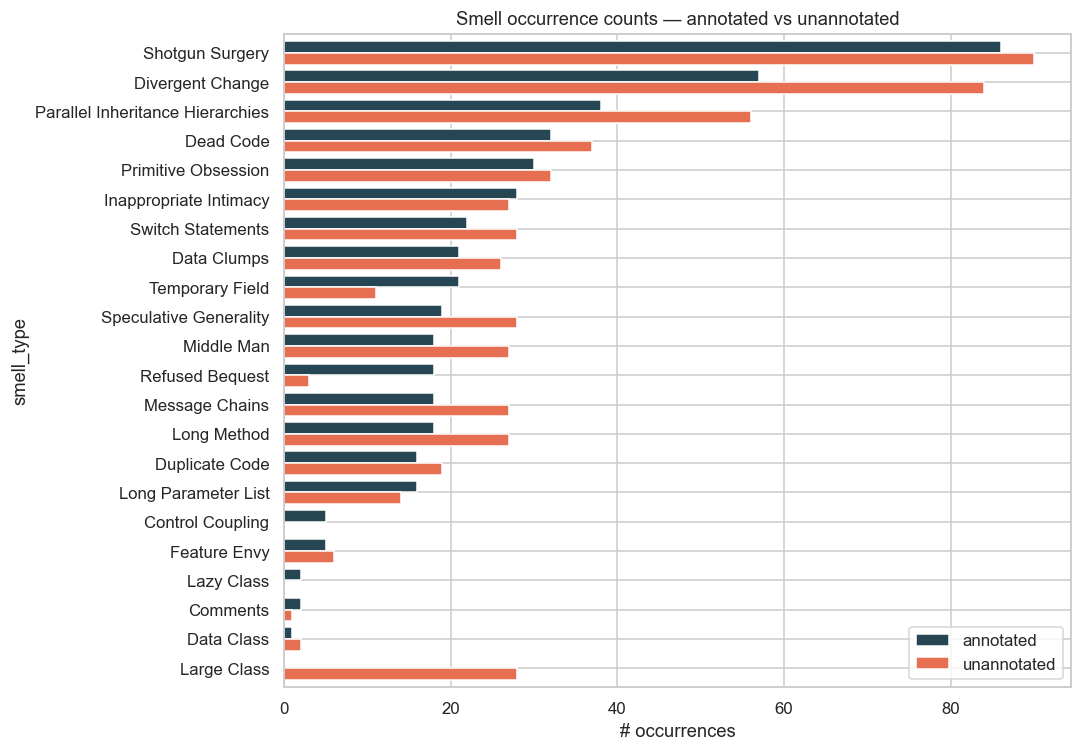
\includegraphics[width=\columnwidth]{03_smell_counts_compare.png}
\caption{Smell-count distribution across the 21 leaf smells. The
distribution is heavy-tailed: \textit{Shotgun Surgery} (86),
\textit{Divergent Change} (57), and \textit{Parallel Inheritance
Hierarchies} (38) dominate, while seven smells have $\le 5$ instances.}
\label{fig:eda-smellcounts}
\end{figure}

\begin{figure}[t]
\centering
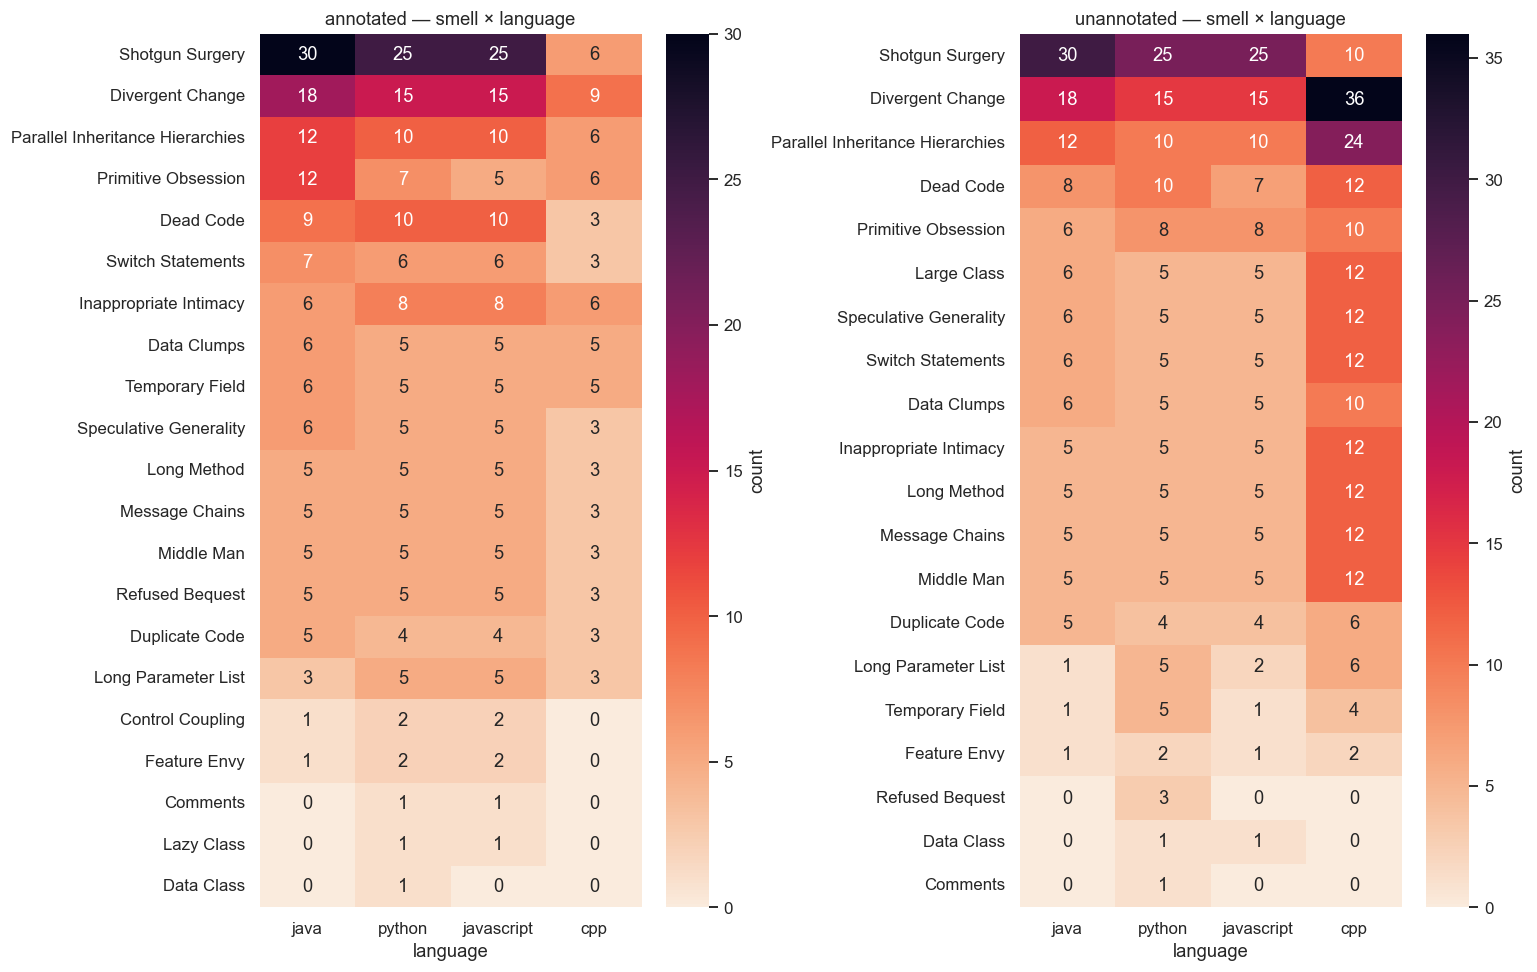
\includegraphics[width=\columnwidth]{04_smell_x_language_heatmap.png}
\caption{Smell $\times$ language heatmap (annotated variant, 473
labels). Coverage is uneven: C++ is sparser per smell while Java,
Python, and JavaScript carry most of the heavy-support smells.}
\label{fig:eda-heatmap}
\end{figure}

\begin{figure}[t]
\centering
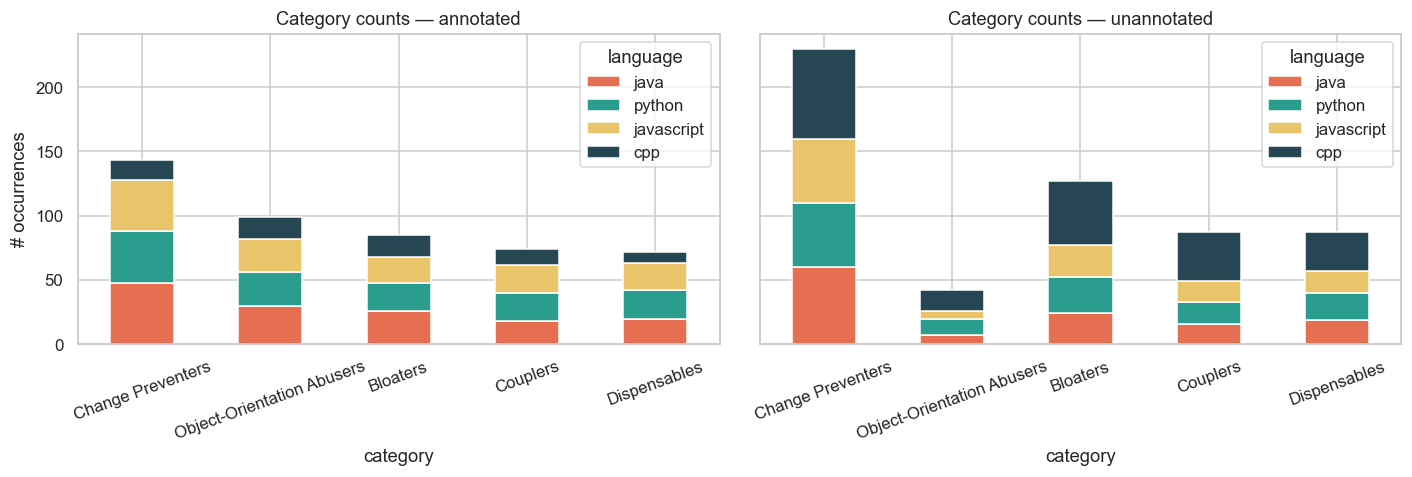
\includegraphics[width=\columnwidth]{05_category_distribution.png}
\caption{Fowler category distribution. \textit{Change Preventers} is
the largest category (143 labels), driven mainly by Shotgun Surgery
and Divergent Change.}
\label{fig:eda-categories}
\end{figure}

\begin{figure}[t]
\centering
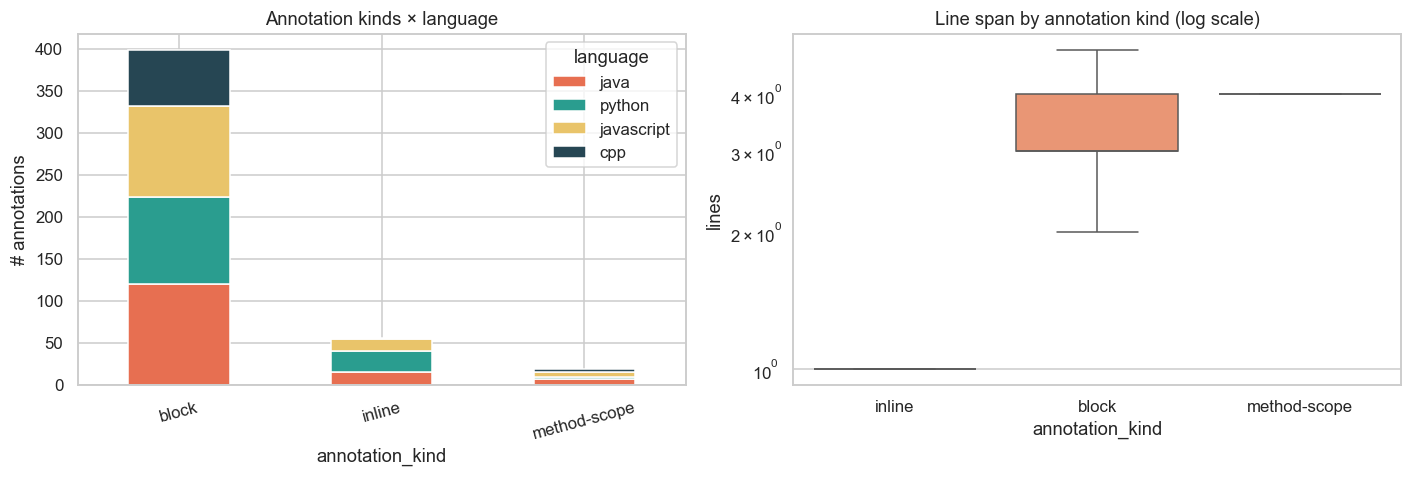
\includegraphics[width=\columnwidth]{06_annotation_kinds.png}
\caption{Annotation kinds: \textit{inline} (single-line),
\textit{block} (comment-introduced multi-line block), and
\textit{method-scope} (extends to method end). The mix matters because
span-overlap matching grants TP credit on $\ge 1$-line overlap.}
\label{fig:eda-kinds}
\end{figure}

\begin{figure}[t]
\centering
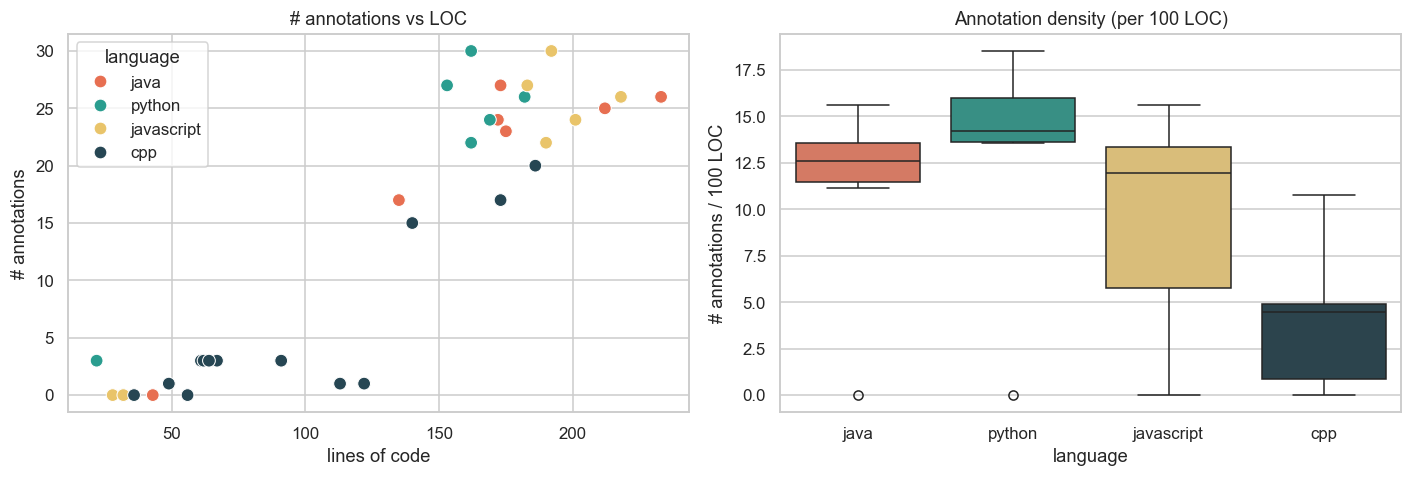
\includegraphics[width=\columnwidth]{07_annotation_density.png}
\caption{Annotation density (smell labels per 100 LOC). Files are
densely annotated by design, every file in the benchmark is a
curated smell exemplar, not a randomly sampled production file.}
\label{fig:eda-density}
\end{figure}

\begin{figure}[t]
\centering
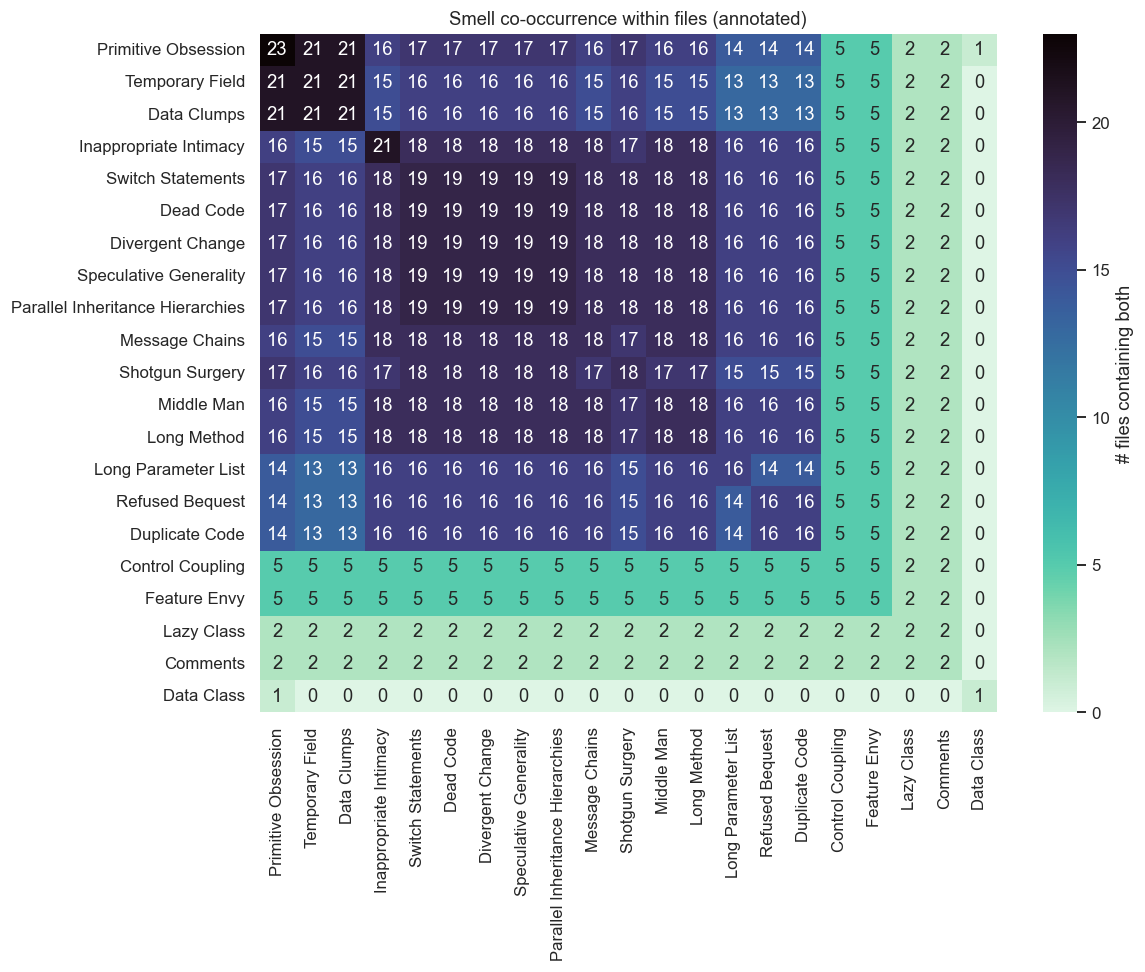
\includegraphics[width=\columnwidth]{08_cooccurrence.png}
\caption{Smell co-occurrence within the same file. Strong co-occurrence
clusters around \textit{Shotgun Surgery / Divergent Change / Parallel
Inheritance Hierarchies}, reflecting the dataset's emphasis on
change-preventer scenarios.}
\label{fig:eda-cooc}
\end{figure}

\begin{figure}[t]
\centering
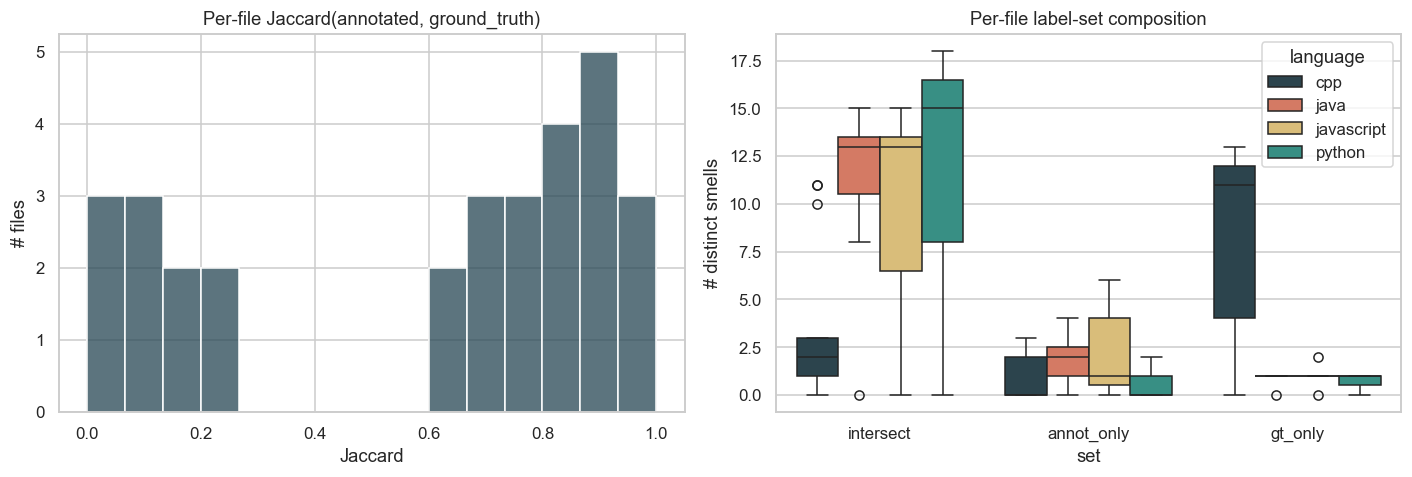
\includegraphics[width=\columnwidth]{09_annot_vs_gt_coverage.png}
\caption{Coverage check: line-level inline annotations (473) vs.\ the
method-level CSV ground truth (573). The two views are consistent up
to granularity differences and the C++ \texttt{.cpp}/\texttt{.h}
split; we use the line-level annotated variant for evaluation.}
\label{fig:eda-coverage}
\end{figure}

\begin{figure}[t]
\centering
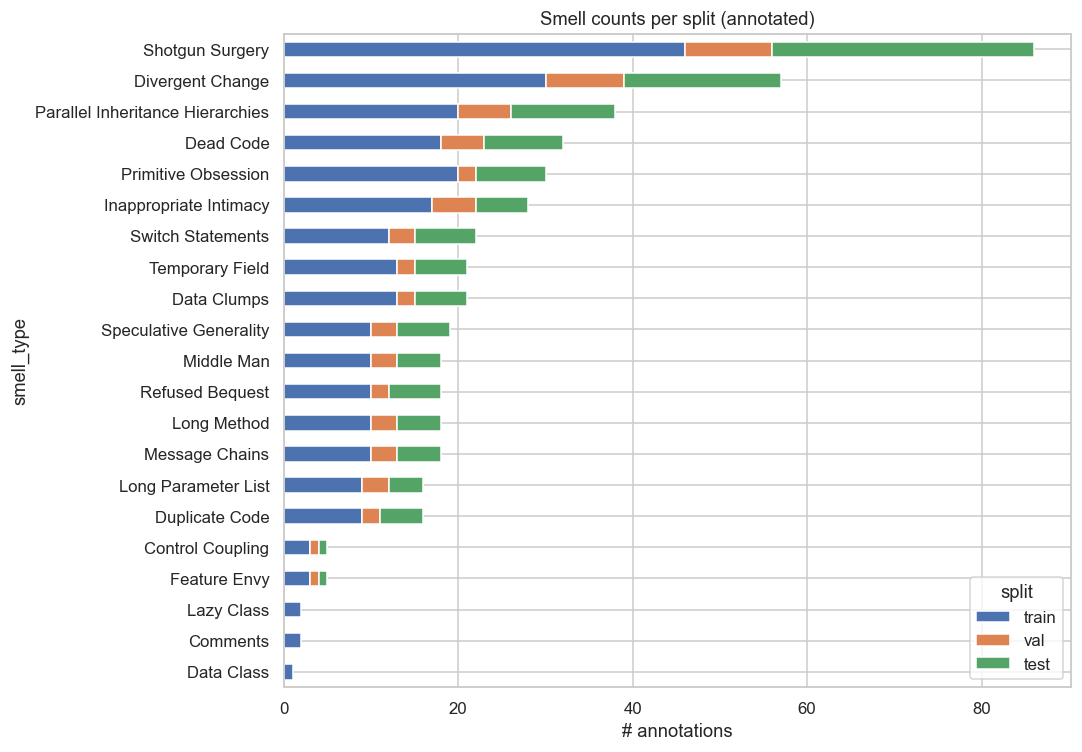
\includegraphics[width=\columnwidth]{10_split_balance.png}
\caption{Train / validation / test split balance per language
(seed=42, 60/20/20). The split is stratified by language; per-smell
stratification is not enforced because long-tail smells have
insufficient support.}
\label{fig:eda-splits}
\end{figure}

\noindent The recurring observation is the \emph{small absolute scale}
(34 files, 473 labels) and the \emph{long-tail label distribution}.
We revisit both as explicit threats in Section~\ref{sec:threats}.

%======================================================================
\section{Methodology}
%======================================================================

\subsection{Dataset}
We use the \textit{Smelly Code Dataset}~\cite{sadik2025smellycode}, an expert-validated
multi-language benchmark of files exhibiting Fowler-style smells. After
harmonization into a unified JSON schema we obtain the \emph{annotated} variant
summarized in Table~\ref{tab:dataset}.

\begin{table}[t]
\centering
\caption{Dataset summary (annotated variant).}
\label{tab:dataset}
\begin{tabular}{lr}
\toprule
\textbf{Property} & \textbf{Value} \\
\midrule
Files (Java / Python / JavaScript / C++) & 7 / 7 / 7 / 13 (\textbf{34}) \\
Train / Val / Test split & 20 / 6 / 8 \\
Total line-level smell labels & 473 \\
Distinct smell types & 21 \\
Fowler categories & 5 \\
Most frequent smell & Shotgun Surgery (86) \\
Largest Fowler category & Change Preventers (143) \\
\bottomrule
\end{tabular}
\end{table}

The annotations span all 21 smell types in the Fowler taxonomy with non-uniform
support: \textit{Shotgun Surgery} (86), \textit{Divergent Change} (57), and
\textit{Parallel Inheritance Hierarchies} (38) dominate, while the long tail
(\textit{Lazy Class}, \textit{Comments}, \textit{Data Class},
\textit{Feature Envy}) has $\le 5$ instances. We report all results pooled across
languages and additionally break out per-language and per-smell behavior.

\subsection{Models Under Test}
All three models are instruction-tuned LLMs whose weights are publicly
published, and are served via AWS Bedrock in \texttt{ap-southeast-2} with
$\text{temperature}{=}0$, $\text{top\_p}{=}1$, and a fixed seed (\texttt{42}).
We therefore characterize the Bedrock-served deployment of these weights;
results on self-hosted inference (different precision, system prompts, or
sampling backends) may differ. The set spans three distinct architectural
points (sparse MoE, small dense, large dense) and three model families:
\begin{itemize}
 \item \textbf{DeepSeek~v3.2~671B}~\cite{deepseekai2024v3}, a large-scale sparse Mixture-of-Experts
 (MoE) model with $\sim$671--685B total parameters and $\sim$37B active per
 token via MoE routing, supporting context lengths up to $\sim$128K tokens.
 Designed for high reasoning performance with strong computational efficiency
 on long-context and agent-style tasks.
 \item \textbf{Gemma 3 27B-IT}~\cite{gemma3team2025}, Google's 27B-parameter \emph{dense}
 instruction-tuned model from the Gemma~3 family, optimized for instruction
 following, reasoning, and cost-efficient single-node GPU inference.
 \item \textbf{Mistral Devstral 2 123B}~\cite{jiang2023mistral}, a 123B-parameter \emph{dense}
 transformer (not MoE) with up to 256K-token context, instruction-tuned
 (Instruct variant) and purpose-built for agentic software-engineering
 tasks including multi-step reasoning, tool use, and large-codebase
 manipulation.
\end{itemize}

\subsection{Prompting Strategies}
We hold the \emph{system message} (task description plus the 21-smell taxonomy)
and \emph{output schema} (structured JSON list of \texttt{(smell, line\_start,
line\_end)} tuples) constant across conditions, varying only the user prompt:
\begin{itemize}
 \item \textbf{P1 Zero-shot}: instruction + code.
 \item \textbf{P2 Few-shot}: P1 + 3 worked in-context
 examples~\cite{brown2020fewshot}.
 \item \textbf{P3 Taxonomy-tree CoT}: P1 + an explicit chain-of-thought walk
 through the 5 Fowler categories before producing the final
 answer~\cite{wei2022cot}.
 \item \textbf{P4 Self-verify}: P1 + a two-stage prompt that (a) produces a
 candidate list, (b) critiques and revises it, in the spirit of
 Self-Refine~\cite{madaan2023selfrefine}.
 \item \textbf{P5 RAG (dense, $k{=}3$)}: P1 + 3 most-similar smell-annotated
 chunks retrieved from a ChromaDB index over the train split using
 sentence-transformer embeddings~\cite{reimers2019sbert}.
 \item \textbf{P5 RAG (random, $k{=}2$, ablation)}: identical prompt template,
 but the ``retrieved'' chunks are sampled uniformly at random from the train
 split. This isolates retrieval \emph{content} from retrieval \emph{length}.
\end{itemize}

\subsection{Variables and Controls}
\textbf{Independent variables:} model (3 levels), prompting strategy (6 levels),
language (4 levels). \textbf{Controls held constant:} system prompt, output
schema, decoding temperature/seed, evaluation split, span-overlap matching policy,
and the ground-truth labels. \textbf{Dependent variables:} per-record TP/FP/FN,
micro precision/recall/F1, macro F1, parse-error rate, wall-clock latency. The
ablation condition (P5 random) varies only the \emph{content} of retrieved chunks
while holding their count and template position constant.

\subsection{Evaluation Pipeline}
Predictions are matched to ground-truth annotations under a span-overlap policy
(predicted span overlaps gold span by $\ge 1$ line and the smell label matches).
For each (model, prompt, language) cell we compute:
\begin{itemize}
 \item \textbf{Micro F1} pooled from raw TP/FP/FN counts.
 \item \textbf{Macro F1} averaged across smell classes (with support).
 \item \textbf{Bootstrap 95\% CI} on micro F1 via 1{,}000 stratified
 resamples~\cite{efron1993bootstrap}.
 \item \textbf{Paired bootstrap}~\cite{efron1993bootstrap} on per-record
 micro F1 differences (paired by
 \texttt{sample\_id}) to test significance of (a)~each prompt vs.~zero-shot
 within a model, (b)~cross-model best-prompt comparisons, and (c)~the dense-
 vs.-random RAG ablation. A 95\% CI on the difference that excludes 0 is
 reported as significant ($\checkmark$).
 \item \textbf{Cost/latency:} wall-clock seconds per language summed across
 the four languages.
\end{itemize}

\subsection{Implementation}
The pipeline is implemented in Python 3.12 (pandas, NumPy, scikit-learn).
Retrieval uses sentence-transformer embeddings persisted in ChromaDB. All
artifacts, prompts (per language), per-record CSVs, per-smell breakdowns, and
the analysis notebook are released in the public repository, enabling
regeneration of every figure in this paper from a single notebook.

%======================================================================
\section{Evaluation}
%======================================================================

\subsection{Headline Results}
Table~\ref{tab:headline} reports pooled micro/macro precision, recall, and F1 for
each of the 18 (model, prompt) cells. The corresponding heatmap and grouped-bar
view appear in Fig.~\ref{fig:headline}.

\begin{table}[t]
\centering
\caption{Headline results: pooled micro precision (P), recall (R), F1, and macro
F1 across all four languages. Best per model is \textbf{bold}; overall best is
\underline{underlined}.}
\label{tab:headline}
\renewcommand{\arraystretch}{1.05}
\begin{tabular}{llcccc}
\toprule
\textbf{Model} & \textbf{Prompt} & \textbf{P} & \textbf{R} & \textbf{F1} & \textbf{Macro F1} \\
\midrule
\multirow{6}{*}{DeepSeek v3.2 671B}
 & P1 zero-shot & 0.776 & 0.769 & 0.773 & 0.777 \\
 & P2 few-shot & 0.901 & 0.812 & \textbf{0.854} & 0.848 \\
 & P3 tax-tree & 0.741 & 0.714 & 0.727 & 0.699 \\
 & P4 self-verify & 0.463 & 0.147 & 0.224 & 0.208 \\
 & P5 RAG dense & 0.878 & 0.769 & 0.820 & 0.784 \\
 & P5 RAG random & 0.882 & 0.797 & 0.837 & 0.802 \\
\midrule
\multirow{6}{*}{Gemma 3 27B-IT}
 & P1 zero-shot & 0.712 & 0.744 & 0.727 & 0.727 \\
 & P2 few-shot & 0.936 & 0.816 & \textbf{0.872} & 0.885 \\
 & P3 tax-tree & 0.739 & 0.690 & 0.714 & 0.715 \\
 & P4 self-verify & 0.635 & 0.487 & 0.551 & 0.569 \\
 & P5 RAG dense & 0.937 & 0.665 & 0.778 & 0.774 \\
 & P5 RAG random & 0.921 & 0.650 & 0.762 & 0.746 \\
\midrule
\multirow{6}{*}{Mistral Devstral 2 123B}
 & P1 zero-shot & 0.696 & 0.688 & 0.692 & 0.770 \\
 & P2 few-shot & 0.953 & 0.942 & 0.947 & 0.927 \\
 & P3 tax-tree & 0.547 & 0.656 & 0.597 & 0.652 \\
 & P4 self-verify & 0.665 & 0.551 & 0.603 & 0.671 \\
 & P5 RAG dense & 0.962 & 0.966 & \underline{\textbf{0.964}} & \textbf{0.943} \\
 & P5 RAG random & 0.939 & 0.927 & 0.933 & 0.876 \\
\bottomrule
\end{tabular}
\end{table}

\begin{figure}[t]
\centering
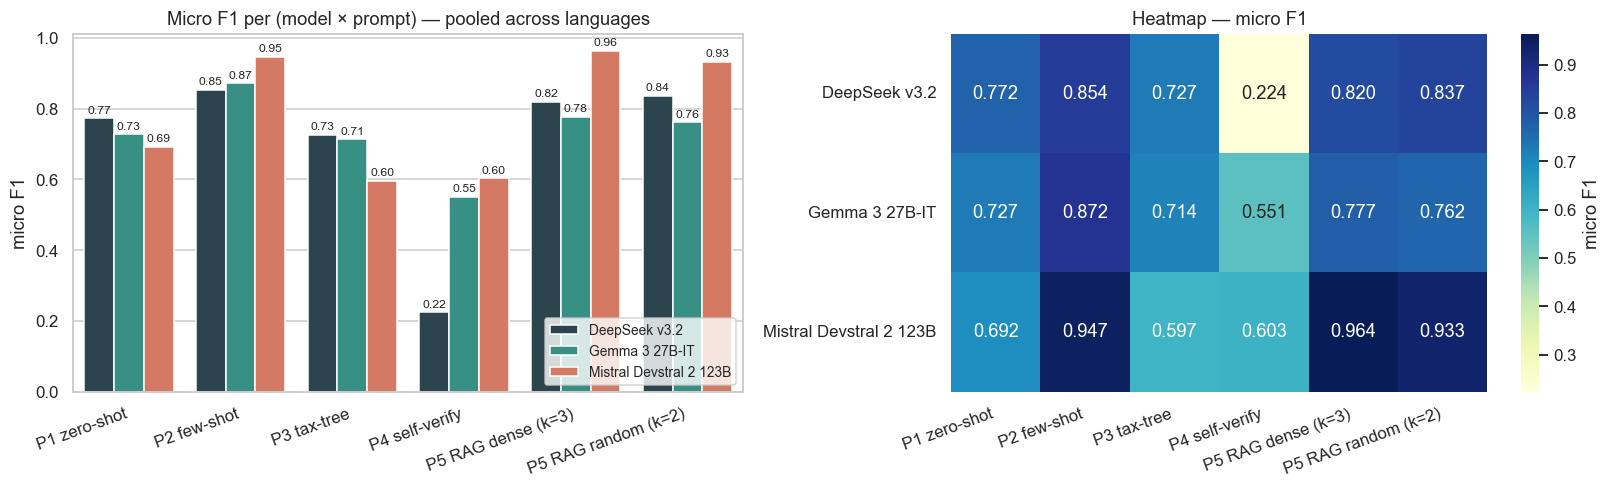
\includegraphics[width=\columnwidth]{02_headline_f1.png}
\caption{Pooled micro F1 across all (model, prompt) cells. Mistral~Devstral~2 with
P5 dense RAG dominates; few-shot is the strongest universal lever; self-verify is
catastrophic for DeepSeek and harmful for Gemma.}
\label{fig:headline}
\end{figure}

\noindent\textbf{Observations.}
(1) The overall best system is \textit{Mistral Devstral 2 123B~+~P5 RAG dense}
(F1$=$0.964). (2) Few-shot is the best prompt for both DeepSeek (0.854) and Gemma
(0.872). (3) Mistral derives further gains from RAG; the smaller models do not.
(4) Self-verify is harmful for every model and ruinous for DeepSeek
($-0.55$ absolute F1 vs.~zero-shot).

\subsection{Leaderboard with Bootstrap CIs}
Fig.~\ref{fig:leaderboard} presents grouped error-bar plots per prompt with
bootstrap CIs averaged over languages. The CIs make explicit that the
Mistral~+~RAG-dense advantage is not driven by a single language.

\begin{figure}[t]
\centering
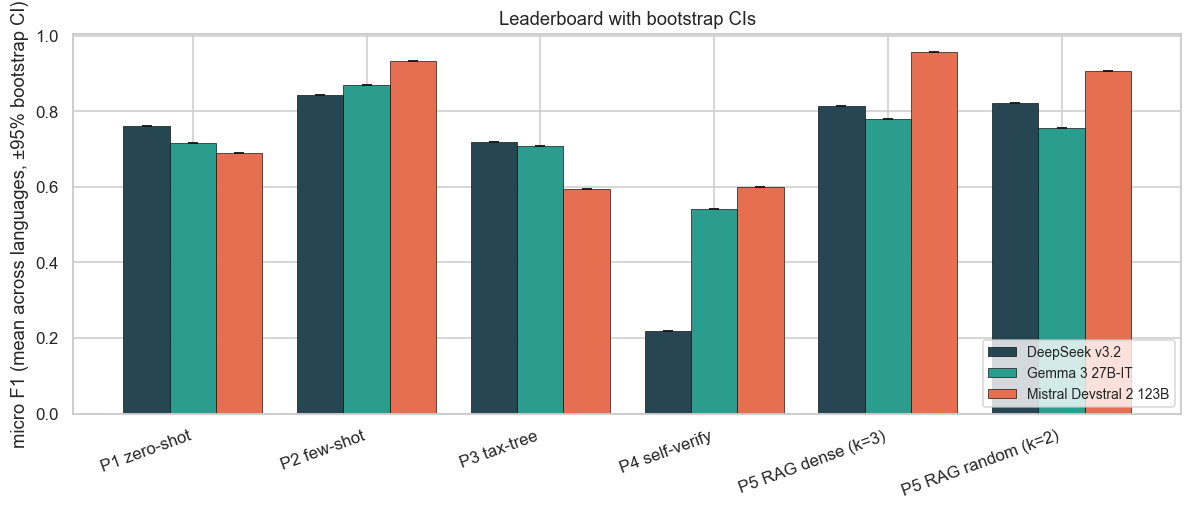
\includegraphics[width=\columnwidth]{03_leaderboard_ci.png}
\caption{Leaderboard with 95\% bootstrap confidence intervals on micro F1
(mean across languages). Mistral's lead under P2 and P5 is robust to resampling.}
\label{fig:leaderboard}
\end{figure}

\subsection{Prompt-Strategy Effect}
Fig.~\ref{fig:delta} shows $\Delta\mathrm{F1}$ vs.~the P1 baseline per model. P2
yields large positive lift uniformly ($+0.08$ to $+0.26$). P3 and P4 are
\emph{negative} across the board. RAG (dense and random) is positive only on
Mistral; on DeepSeek and Gemma the RAG variants are roughly neutral or slightly
positive but with overlapping CIs.

\begin{figure}[t]
\centering
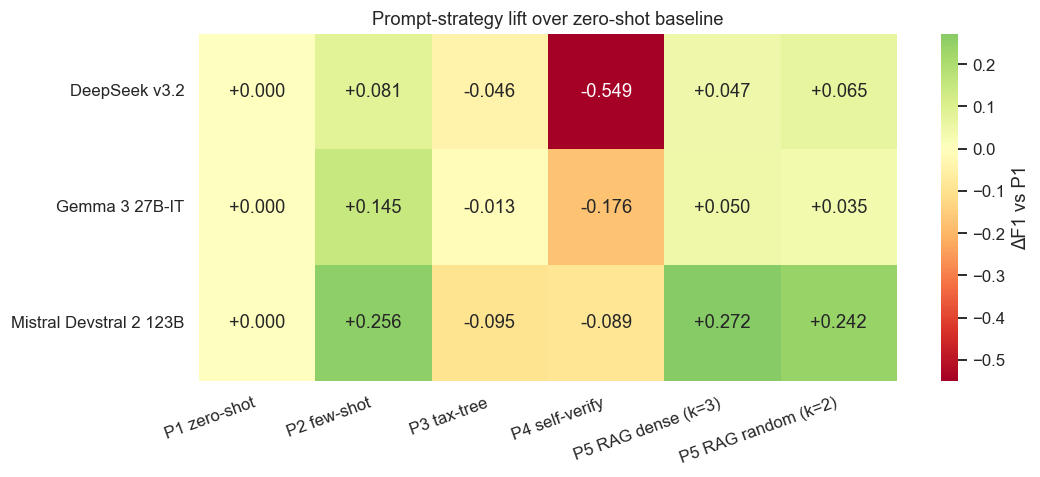
\includegraphics[width=\columnwidth]{04_delta_vs_p1.png}
\caption{$\Delta$F1 over zero-shot baseline per (model, prompt). Greens are
improvements, reds are regressions.}
\label{fig:delta}
\end{figure}

\subsection{Statistical Significance}
We report paired-bootstrap CIs on per-record F1 differences. Out of 15
within-model prompt-vs.-P1 comparisons, 9 are significant
(Table~\ref{tab:within}). Cross-model, Mistral~+~RAG-dense significantly beats
both other models at their respective best prompts (Table~\ref{tab:cross}).

\begin{table}[t]
\centering
\caption{Paired-bootstrap 95\% CI on $\Delta$F1 vs.~P1 zero-shot, within model
($n_{\text{boot}}{=}1000$, paired by record). \checkmark{} indicates the CI
excludes 0.}
\label{tab:within}
\begin{tabular}{llrrrc}
\toprule
\textbf{Model} & \textbf{Comparison} & $\Delta$F1 & CI low & CI high & \textbf{Sig} \\
\midrule
\multirow{5}{*}{DeepSeek v3.2 671B}
 & P2 vs P1 & 0.081 & 0.003 & 0.176 & \checkmark \\
 & P3 vs P1 & -0.046 & -0.104 & 0.018 & ns \\
 & P4 vs P1 & -0.549 & -0.682 & -0.392 & \checkmark \\
 & P5d vs P1 & 0.048 & -0.009 & 0.111 & ns \\
 & P5r vs P1 & 0.065 & 0.004 & 0.136 & \checkmark \\
\midrule
\multirow{5}{*}{Gemma 3 27B-IT}
 & P2 vs P1 & 0.145 & 0.054 & 0.255 & \checkmark \\
 & P3 vs P1 & -0.013 & -0.082 & 0.069 & ns \\
 & P4 vs P1 & -0.176 & -0.275 & -0.077 & \checkmark \\
 & P5d vs P1 & 0.050 & -0.047 & 0.158 & ns \\
 & P5r vs P1 & 0.035 & -0.080 & 0.162 & ns \\
\midrule
\multirow{5}{*}{Mistral Devstral 2 123B}
 & P2 vs P1 & 0.256 & 0.184 & 0.336 & \checkmark \\
 & P3 vs P1 & -0.095 & -0.166 & -0.018 & \checkmark \\
 & P4 vs P1 & -0.089 & -0.218 & 0.019 & ns \\
 & P5d vs P1 & 0.272 & 0.191 & 0.365 & \checkmark \\
 & P5r vs P1 & 0.242 & 0.154 & 0.337 & \checkmark \\
\bottomrule
\end{tabular}
\end{table}

\begin{table}[t]
\centering
\caption{Cross-model paired bootstrap at each model's best prompt.}
\label{tab:cross}
\begin{tabular}{p{2.6cm}p{2.6cm}rc}
\toprule
\textbf{A} & \textbf{B} & \textbf{$\Delta$F1 (B$-$A)} & \textbf{Sig} \\
\midrule
DeepSeek (P2) & Gemma (P2) & 0.018 & ns \\
DeepSeek (P2) & Mistral (P5 dense) & 0.110 & \checkmark \\
Gemma (P2) & Mistral (P5 dense) & 0.092 & \checkmark \\
\bottomrule
\end{tabular}
\end{table}

\subsection{RAG Content vs.~Length Ablation}
Table~\ref{tab:rag} and Fig.~\ref{fig:rag} present the dense-vs.-random retrieval
ablation. The content effect is positive but small for Gemma and Mistral and
slightly negative for DeepSeek. Only Mistral's $+0.030$ dense-over-random lift is
statistically significant (CI $[0.002, 0.069]$).

\begin{table}[t]
\centering
\caption{RAG ablation: dense ($k{=}3$) minus random ($k{=}2$) retrieval, per
model.}
\label{tab:rag}
\begin{tabular}{lrrrc}
\toprule
\textbf{Model} & \textbf{$\Delta$F1} & \textbf{CI low} & \textbf{CI high} & \textbf{Sig} \\
\midrule
DeepSeek v3.2 671B & -0.017 & -0.067 & 0.029 & ns \\
Gemma 3 27B-IT & 0.016 & -0.046 & 0.098 & ns \\
Mistral Devstral 2 123B& 0.031 & 0.002 & 0.069 & \checkmark \\
\bottomrule
\end{tabular}
\end{table}

\begin{figure}[t]
\centering
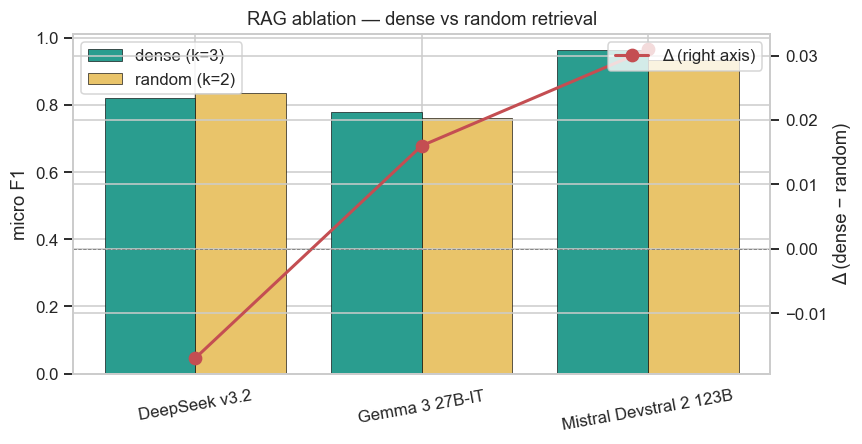
\includegraphics[width=\columnwidth]{05_rag_ablation.png}
\caption{Dense (k=3) vs.\ random (k=2) retrieval per model; right axis shows the
content delta. Only Mistral exhibits a statistically significant content effect.}
\label{fig:rag}
\end{figure}

\subsection{Per-Language Sensitivity}
Fig.~\ref{fig:perlang} plots micro F1 per (prompt, language) for each model.
Difficulty ranking averaged across all (model, prompt) cells is
\textbf{Python (0.81) $>$ JavaScript (0.76) $>$ Java (0.71) $>$ C++ (0.65)}.
Mistral closes the C++ gap markedly under RAG-dense ($0.899$) but the smaller
models still underperform on C++ where retrieval evidence appears most beneficial.

\begin{figure*}[t]
\centering
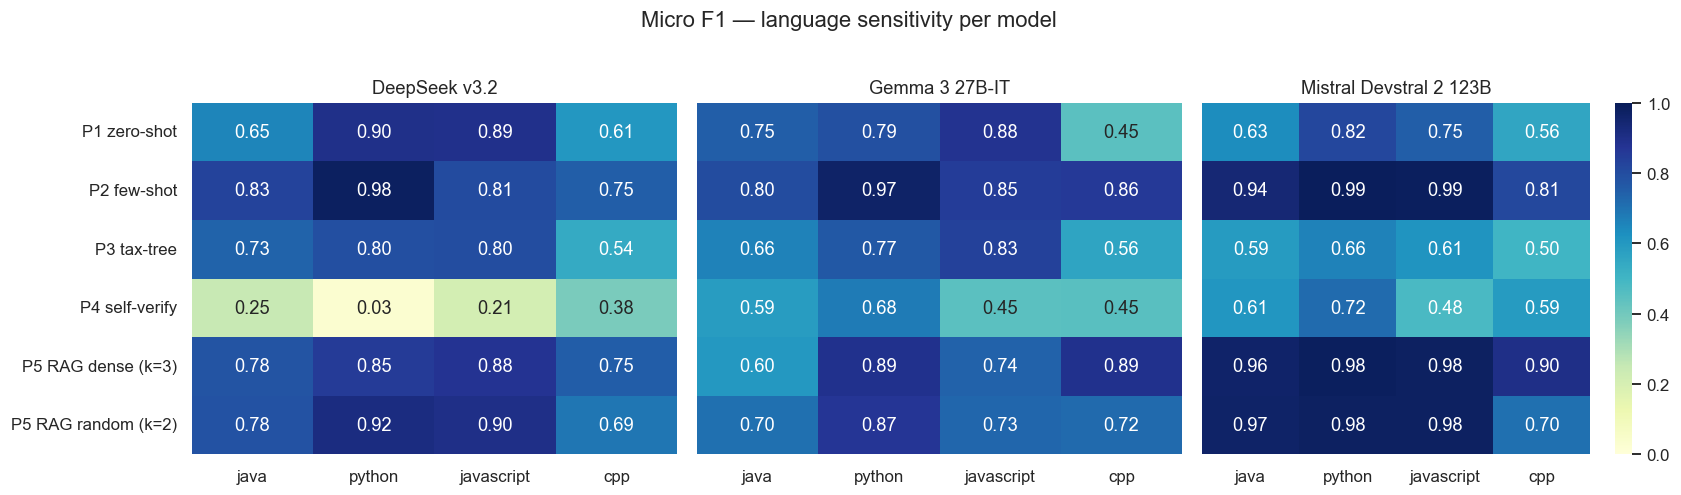
\includegraphics[width=\textwidth]{06_per_language_heatmaps.png}
\caption{Per-language F1 heatmaps (one per model). Rows are prompt strategies,
columns are languages. Mistral's RAG-dense row is uniformly bright; the smaller
models show high variance on C++.}
\label{fig:perlang}
\end{figure*}

\subsection{Per-Smell Behavior}
Using each model's best prompt, we pool TP/FP/FN per smell across languages
(Fig.~\ref{fig:persmell}). High-support smells (\textit{Shotgun Surgery},
\textit{Dead Code}, \textit{Primitive Obsession}) are detected reliably
($\ge 0.93$ F1) by all models. Mistral hits perfect F1 on six smell types
(\textit{Divergent Change}, \textit{Dead Code}, \textit{Inappropriate Intimacy},
\textit{Speculative Generality}, \textit{Long Method}, \textit{Feature Envy}).
The hardest smells (mean F1 across models, $\text{support}{\ge}10$) are
\textit{Parallel Inheritance Hierarchies} (0.78), \textit{Divergent Change}
(0.80), \textit{Switch Statements} (0.80), \textit{Long Parameter List} (0.81),
and \textit{Refused Bequest} (0.81), all of which require multi-class or
cross-file reasoning.

\begin{figure}[t]
\centering
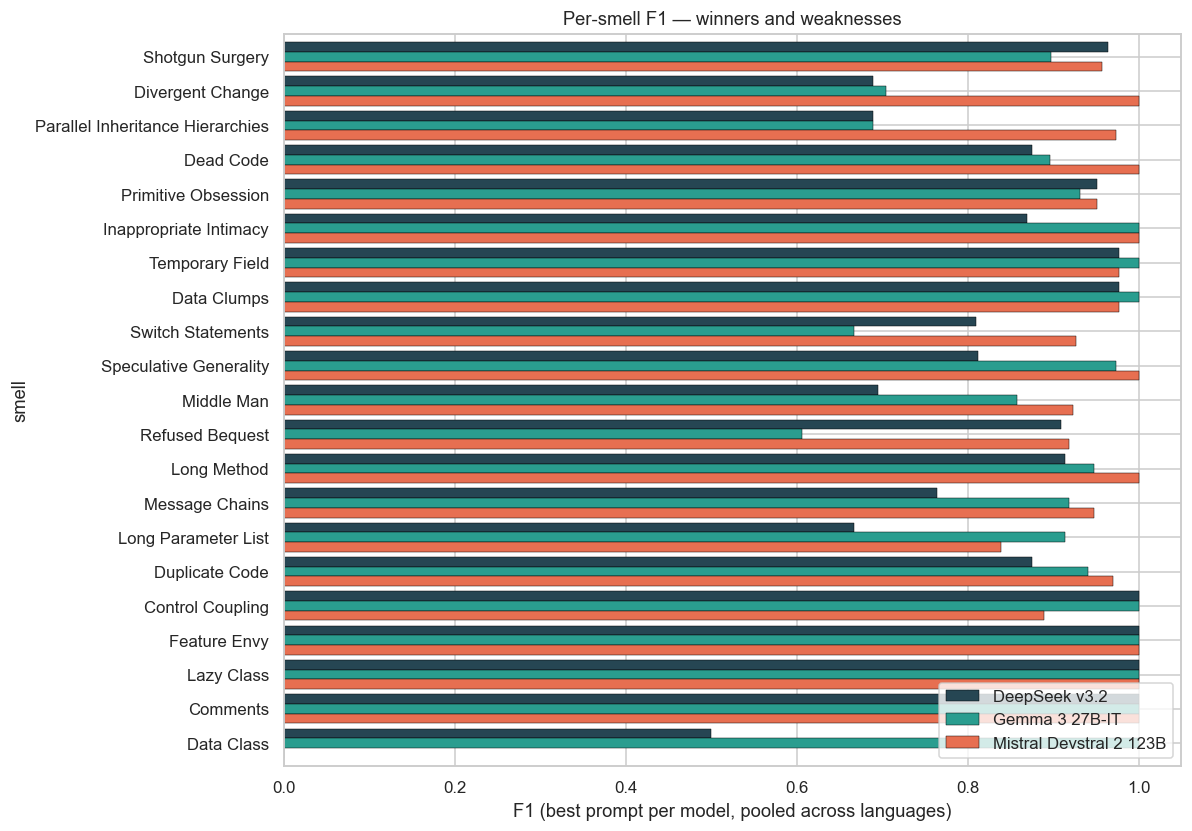
\includegraphics[width=\columnwidth]{07_per_smell_f1.png}
\caption{Per-smell F1 at each model's best prompt. Mistral is at or near 1.0 on
most high-support smells; the smaller models lag on inheritance- and
coupling-heavy smells.}
\label{fig:persmell}
\end{figure}

\subsection{Error Mix and Output Reliability}
Fig.~\ref{fig:errmix} decomposes total findings into TP/FP/FN per cell and shows
the JSON output-format error rate. Two patterns dominate: (i)~self-verify (P4)
collapses recall and creates a disproportionately FN-heavy error mix
(Mistral~P4: 210 FN vs.\ 130 FP; DeepSeek~P4: 399 FN); (ii)~JSON parse failures
are concentrated in P4 (DeepSeek 9.3\%, Mistral 0.5\%, Gemma 0.3\%); all other
prompts produce 0\% parse errors. Mistral's RAG-dense run reaches a 1.12 FP/FN
balance with only 18 FP and 16 FN out of 470 findings, the cleanest output mix
in the experiment.

\begin{figure}[t]
\centering
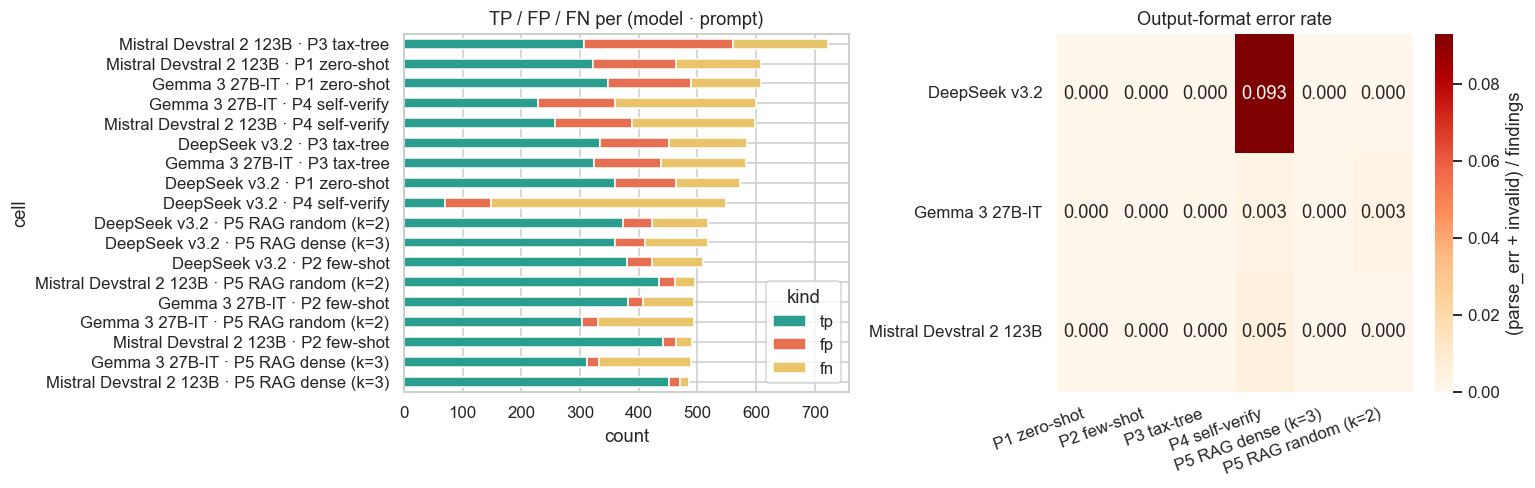
\includegraphics[width=\columnwidth]{08_error_mix.png}
\caption{Left: stacked TP/FP/FN per (model, prompt). Right: JSON output-format
error rate; only P4 self-verify produces non-zero parse failures.}
\label{fig:errmix}
\end{figure}

\subsection{Cost / Latency Trade-off}
Fig.~\ref{fig:cost} plots F1 against total wall-clock seconds across the four
languages (log-scaled). The Pareto frontier is dominated by Mistral~+~RAG-dense
(F1$=$0.964 in 584~s) and Mistral~+~P2 (F1$=$0.947 in 534~s). P4 self-verify is
strictly dominated everywhere: it is both the slowest (DeepSeek P4: 5{,}401~s,
$9.3\times$ slower than its P1) and the least accurate.

\begin{figure}[t]
\centering
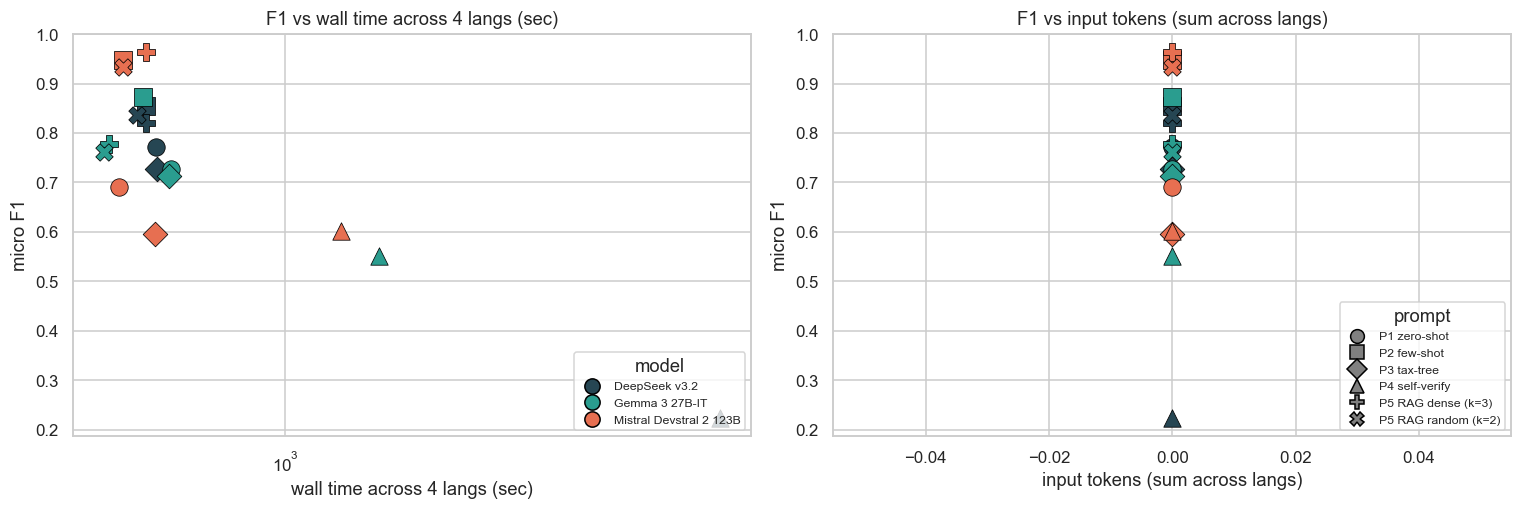
\includegraphics[width=\columnwidth]{09_cost_vs_f1.png}
\caption{F1 vs.\ wall-clock time (log axis). The upper-left frontier is occupied
exclusively by Mistral; self-verify is Pareto-dominated for every model.}
\label{fig:cost}
\end{figure}

%======================================================================
\section{Results Analysis}
%======================================================================

\subsection{RQ1, Few-shot vs.\ Zero-shot}
Few-shot prompting (P2) is the most reliable single intervention in our study.
It improved F1 over P1 \textbf{for every model} (DeepSeek $+0.081$,
Gemma $+0.145$, Mistral $+0.256$) and is statistically significant for every
model (Table~\ref{tab:within}). Mean lift across the three models is $+0.161$
F1. The strongest beneficiary is the largest model, suggesting that few-shot
demonstrations help most when the underlying capacity to imitate structured
exemplars is high. \textbf{Answer to RQ1:} \emph{Yes}, in-context demonstration
is unambiguously the strongest universal lever for this task.

\subsection{RQ2, Structured Reasoning Prompts}
Both structured-reasoning prompts \emph{hurt} accuracy on average. P3
taxonomy-tree mean lift is $-0.051$ F1 and P4 self-verify mean lift is $-0.271$
F1. Three explanations are consistent with the data:
\begin{itemize}
 \item \textbf{Verification bias.} P4 reduces recall sharply
 (Mistral: 0.942 $\to$ 0.551; DeepSeek: 0.769 $\to$ 0.147). The critique
 stage appears to over-prune candidate findings: ``when in doubt, drop it.''
 \item \textbf{Over-categorization.} P3 forces the model to commit to a
 Fowler category before naming a smell. Misclassification at the category
 step propagates to the smell step. This is most visible on
 \textit{Mistral~P3} where FP nearly doubles (254 FP vs.\ 141 in P1) and
 many findings are tagged with the wrong category.
 \item \textbf{JSON brittleness.} Multi-stage prompts cause more parse
 failures (Fig.~\ref{fig:errmix}) and partial outputs.
\end{itemize}
\noindent\textbf{Answer to RQ2:} \emph{No}, neither structured chain-of-thought
nor self-verification helps on this task; both strategies degrade detection,
sometimes catastrophically.

\subsection{RQ3, Does Retrieval Content Matter?}
The dense-vs.-random ablation provides clean evidence that on smaller
open-weight models (DeepSeek and Gemma)\footnote{We use ``open-weight''
here only to denote that the underlying model weights are publicly
published; our measurements are taken on the Bedrock-served deployment.},
the \emph{presence} of in-context
examples explains nearly all of the RAG benefit; the \emph{specific identity}
of those examples does not (Table~\ref{tab:rag}, ns for both). On Mistral the
content effect is real but modest ($+0.031$, significant). This is consistent
with a two-stage account: the shared system-prompt taxonomy already specifies
the task, and the smaller models have already saturated what they can learn
from the prompt. Larger, code-specialized models can additionally exploit the
precise patterns in dense-retrieved snippets. \textbf{Answer to RQ3:}
\emph{Partially}, retrieval content matters significantly only for the
largest, code-specialized model.

\subsection{Strengths}
The strongest configuration (Mistral~+~P5 dense) achieves \textbf{F1$=$0.964
with P$=$0.962 and R$=$0.966 on this benchmark}, a balanced operating point
on the SmellyCode test split. The evaluation pipeline runs with
deterministic decoding ($T{=}0$, fixed seed) and the underlying model
weights are publicly published, so the same configuration could in
principle be re-deployed on private infrastructure (self-hosted GPU
clusters or VPC-isolated managed endpoints) for privacy-sensitive enterprise
settings, subject to the deployment-equivalence threat noted in
Section~\ref{sec:threats}.

\subsection{Weaknesses}
Three weaknesses are visible in the data:
\begin{itemize}
 \item \textbf{Long-tail smells are unstable.} Smells with $<5$ ground-truth
 instances (\textit{Lazy Class}, \textit{Comments}, \textit{Data Class})
 yield F1 estimates that swing between 0 and 1 across models, uninformative
 at this sample size.
 \item \textbf{C++ underperformance on smaller models.} Gemma~P5-random and
 DeepSeek~P5-dense both fall below 0.7 on C++. Header/template patterns
 appear to be poorly represented in their training data; dense retrieval
 helps Mistral close this gap ($+0.195$ over random) but is too noisy on
 smaller models.
 \item \textbf{Self-verify destroys recall.} Without instruction tuning to
 \emph{revise upward} as well as downward, the critique step systematically
 deletes valid candidates.
\end{itemize}

\subsection{Unexpected Outcomes}
We highlight three results that contradicted our prior expectations:
\begin{enumerate}
 \item \textbf{Random retrieval is competitive on smaller models.} On
 DeepSeek, the ``placebo'' P5 random outperforms the carefully engineered
 P5 dense ($0.837$ vs.\ $0.820$). The simplest interpretation is that any
 extra in-context code primes the model into a structured-output regime;
 the specific code matters little.
 \item \textbf{Chain-of-thought \emph{hurt}.} The widely held intuition
 that CoT helps on classification tasks does not survive contact with this
 benchmark. Forcing an explicit Fowler-category walk before answering
 increases false positives without improving recall.
 \item \textbf{Self-verify is the single worst intervention.} Despite being
 a natural fit for an analyzer-style task, P4 collapses DeepSeek's F1 from
 $0.773$ to $0.224$. The two-stage prompt apparently shifts the model into
 a pathologically conservative mode.
\end{enumerate}

%======================================================================
\section{Threats to Validity}
\label{sec:threats}
%======================================================================

\subsection{Internal Validity}
We mitigate run-to-run nondeterminism by running every model with $T{=}0$ and
a fixed seed (\texttt{42}), and every comparison uses paired records. The
bootstrap on per-record F1 differences accounts for the small ($n{=}34$)
file-level sample size. Remaining threats: AWS Bedrock may be subject to
upstream stochasticity not fully controlled by our seed; we mitigate by
reporting CIs rather than point estimates. A second concern is that our
span-overlap matching grants TP credit when the predicted span covers a gold
span by $\ge 1$ line; tighter matching policies would likely lower all
reported F1 numbers uniformly but should not change the ordering.

\subsection{External Validity}
Our benchmark contains 34 files across 4 languages and 473 line-level
annotations. Findings on smell classes with $<10$ instances are not
generalizable. The dataset is expert-validated but small; results on
industrial-scale code with thousands of files may differ, particularly for
smells like \textit{Large Class} that depend on file-scale context. We
evaluate three models from three families; results on other LLMs (e.g.,
GPT-4-class commercial APIs, Code Llama, smaller 7B--13B variants) are not
directly transferable.

\subsection{Construct Validity}
F1 over span-matched annotations operationalizes ``correct smell detection''
as ``predicted smell label and span overlap a gold annotation.'' This rewards
near-correct localization but penalizes annotation-style differences (e.g.,
method-level vs.\ line-level granularity). We additionally report per-smell F1
and error-mix breakdowns to expose where the metric may mislead. Our
random-retrieval control isolates content from length but not from
\emph{topic}; random examples are still drawn from the same domain (annotated
smelly code), so any priming effect is domain-specific. A truly
content-agnostic control would draw from out-of-domain code, which we leave
to future work.

\subsection{Limitations Not Addressed in This Study}
For full transparency we list controls that a stronger version of this
study should add but that we did \emph{not} run here:
\begin{itemize}
 \item \textbf{Data-contamination probe.} The Smelly Code Dataset is
 publicly hosted on GitHub; the three models were trained on
 web-scale code corpora. We did not run a membership-inference-style
 completion probe to estimate the chance that any benchmark file is
 memorised. Numbers near 1.0 should be read with this in mind.
 \item \textbf{Retrieval-leakage check.} The dense RAG index and the
 test split are both drawn from the same 34-file corpus. We did not
 quantify the maximum embedding similarity between each test chunk
 and its top-1 retrieved neighbour; high similarity would inflate
 the apparent retrieval lift on Mistral.
 \item \textbf{Multi-seed / multi-paraphrase variance.} We ran one
 decoding pass per (model, prompt, language) cell at $T{=}0$,
 seed=42. Bedrock greedy decoding is not bit-reproducible across
 calls in our experience, but we did not measure the resulting
 variance with repeat runs or paraphrased prompts.
 \item \textbf{Deployment equivalence.} Bedrock-served inference may
 differ from self-hosted inference (precision, system prompts,
 safety filters, sampling backend). Numbers reported here
 characterize the Bedrock deployment of the listed model versions.
 \item \textbf{Fine-tuned encoder baseline.} A directly comparable
 fine-tuned classifier (e.g., CodeBERT/CodeT5/UniXcoder) was not
 trained for this study.
 \item \textbf{Qualitative error analysis.} We report per-smell F1
 and TP/FP/FN counts but do not include a manual categorisation of
 a held-out sample of false positives and false negatives.
\end{itemize}
Each of these is a plausible avenue for follow-up work and is
consistent with the headline number being treated as an upper bound
rather than a population-level estimate.

%======================================================================
\section{Conclusion and Future Work}
\label{sec:conclusion}
%======================================================================

We presented a controlled empirical evaluation of three instruction-tuned
LLMs (served via AWS Bedrock) across five prompting strategies (plus a
random-retrieval ablation) on an expert-validated, multi-language
code-smell benchmark. On this benchmark the strongest
configuration, \textit{Mistral Devstral 2 123B} with dense
retrieval-augmented prompting, reaches \textbf{micro F1$=$0.964}, a
$+0.272$ absolute lift over zero-shot (95\% CI $[0.191, 0.365]$, paired
bootstrap), and significantly beats both other models at their best
prompt. We treat this as a benchmark-specific upper bound for this
configuration rather than a population-level accuracy estimate (see
Section~\ref{sec:threats}). We provide three actionable
findings:
\begin{enumerate}
 \item \textbf{Always use few-shot.} P2 yields significant gains for every
 model (mean $+0.161$ F1) and is the single best universal intervention.
 \item \textbf{Avoid taxonomy-tree CoT and self-verify on this task.} Both
 degrade accuracy; self-verify can be catastrophic.
 \item \textbf{Use dense RAG only on large code-specialized models.} For
 smaller models, retrieval \emph{length} explains nearly all of the
 benefit; retrieval \emph{content} matters significantly only for Mistral.
\end{enumerate}

\paragraph*{Future work} extends in two directions. First, we plan to scale
the benchmark to industrial-size repositories (10k+ files) and incorporate
\textit{Large Class} and \textit{God Object} smells whose detection requires
file- or repository-scale context. Second, we will train a directly
comparable fine-tuned encoder baseline (e.g., CodeBERT/CodeT5/UniXcoder)
on the same train/validation split and measure multi-seed variance for
the LLM configurations to convert the headline F1 into a population-level
estimate with confidence intervals across decoding runs.

%======================================================================
\section*{Reproducibility}
All prompts, datasets, predictions, and analysis notebooks are released
in the public GitHub repository at
\url{https://github.com/bibekgupta3333/code-smell/}.
Every figure and table in this paper is regenerated from the released
artifacts by the analysis notebook included in that repository.

\bibliographystyle{IEEEtran}
\bibliography{references}

%======================================================================
\appendices
%======================================================================

\section{Prompt Templates}
\label{app:prompts}

This appendix reproduces the prompt templates used for each of the five
strategies (P1--P5) plus the random-retrieval ablation. The shared
\textit{system message}, \textit{taxonomy block}, and \textit{output schema}
are concatenated at the placeholders \texttt{\{SYSTEM\_BLOCK\}},
\texttt{\{TAXONOMY\}}, and \texttt{\{OUTPUT\_SCHEMA\}} respectively. Per-file
inputs (\texttt{FILE\_PATH}, \texttt{CLASS\_NAME}, \texttt{SOURCE\_CODE}) are
substituted at runtime. Templates are shown in their Python variant; the
Java, JavaScript, and C++ variants differ only in the
``Language-specific guidance'' block and the source-code fence.

\subsection{Shared System Message}

\begin{quote}\small\ttfamily
You are a static-analysis assistant specialised in detecting code smells as
defined by Fowler (\textit{Refactoring}, 2nd ed., 2018).\\[0.3em]
\textbf{Operating principles:}\\
1. \textit{Authority}, use the 23-smell Fowler taxonomy exactly; do not
invent names or merge categories.\\
2. \textit{Evidence-first}, every finding must cite specific lines.\\
3. \textit{Precision over recall}, when uncertain, omit. False positives
are penalised equally to false negatives.\\
4. \textit{Determinism}, same input must produce same output.\\
5. \textit{Format discipline}, final answer is a single JSON object;
no prose, no markdown fences.\\
6. \textit{Abstention}, an empty \texttt{findings} array is a valid,
expected answer for clean code.
\end{quote}

\subsection{Shared Taxonomy Block}

\noindent The 23-smell, 5-category Fowler taxonomy is concatenated at every
\texttt{\{TAXONOMY\}} placeholder. Models must emit \emph{exact} string
matches; common variants (e.g.\ \textit{Message Chain} vs.\ the canonical
\textit{Message Chains}) are scored as misses.

\begin{quote}\small
\textbf{Bloaters} ,
\textit{Long Method} (body $>\,{\sim}25$~LOC or $>\,1$ task);
\textit{Large Class} ($>\,{\sim}10$ fields or $>\,{\sim}15$ methods or
$>\,{\sim}200$~LOC);
\textit{Primitive Obsession} (primitives where a small object/enum would
be clearer);
\textit{Long Parameter List} ($\ge\,4$ params, or $\ge\,3$ of same type);
\textit{Data Clumps} (same field group appearing together repeatedly).

\textbf{Object-Orientation Abusers} ,
\textit{Switch Statements} (long switch/if-else chain on type code);
\textit{Temporary Field} (field meaningful only in some states);
\textit{Refused Bequest} (subclass ignores or no-ops inherited members);
\textit{Alternative Classes with Different Interfaces} (similar work,
divergent signatures);
\textit{Parallel Inheritance Hierarchies} (adding to hierarchy A forces
addition to B).

\textbf{Change Preventers} ,
\textit{Divergent Change} (one class changes for many unrelated reasons);
\textit{Shotgun Surgery} (one change touches many classes).

\textbf{Dispensables} ,
\textit{Comments} (explaining \emph{what} rather than \emph{why});
\textit{Duplicate Code} (near-identical block in $\ge\,2$ places);
\textit{Lazy Class} (does almost nothing);
\textit{Data Class} (only fields + getters/setters);
\textit{Dead Code} (never used or unreachable);
\textit{Speculative Generality} (abstraction without a current user).

\textbf{Couplers} ,
\textit{Feature Envy} (method uses another class's data more than its own);
\textit{Inappropriate Intimacy} (two classes access each other's private
state);
\textit{Message Chains} (\texttt{a.getB().getC().getD()});
\textit{Middle Man} (class whose methods only delegate);
\textit{Control Coupling} (passing a flag that selects callee branch).
\end{quote}

\noindent \textbf{Special markers.} For class-level smells (Large Class,
Lazy Class, Data Class, Alternative Classes), set
\texttt{method = "Entire Class"}.

\subsection{Shared Output Schema}

\begin{quote}\small\ttfamily
Return a single JSON object:\\
\{\\
\hspace*{1em}"language": "java | python | javascript | cpp",\\
\hspace*{1em}"file\_path": "<echo>",\\
\hspace*{1em}"class\_name": "<top-level class or module>",\\
\hspace*{1em}"findings": [ \{\\
\hspace*{2em}"smell\_type": "<one of 23 leaf names>",\\
\hspace*{2em}"category": "Bloaters | OO-Abusers | Change Preventers |\\
\hspace*{3em}Dispensables | Couplers",\\
\hspace*{2em}"method": "<name or 'Entire Class'>",\\
\hspace*{2em}"line\_start": <int>, "line\_end": <int>,\\
\hspace*{2em}"evidence": "<$\le$25 words citing specific code>"\\
\hspace*{1em}\} ]\\
\}
\end{quote}

\noindent Rules: empty \texttt{findings} allowed; no duplicate
\texttt{(method, smell\_type)}; \texttt{smell\_type} is a leaf (never a
category); lines are 1-indexed inclusive; cap of 50 findings per file.

\subsection{P1, Zero-Shot}

\begin{quote}\small\ttfamily
\{SYSTEM\_BLOCK\}\\
\{TAXONOMY\}\\
\{OUTPUT\_SCHEMA\}\\[0.3em]
\textbf{\#\# Task}\\
Detect every code smell in the Python source file below. Apply the
taxonomy and the output schema exactly. Emit JSON only.\\[0.3em]
\textbf{\#\# Input}\\
- language: python\\
- file\_path: \{FILE\_PATH\}\\
- class\_name: \{CLASS\_NAME\}\\[0.3em]
\texttt{```python}\\
\{SOURCE\_CODE\}\\
\texttt{```}\\[0.3em]
Respond with the JSON object only.
\end{quote}

\subsection{P2, Few-Shot (3 worked examples)}

\begin{quote}\small\ttfamily
\{SYSTEM\_BLOCK\} / \{TAXONOMY\} / \{OUTPUT\_SCHEMA\}\\[0.3em]
\textbf{\#\# Task}\\
Detect every code smell in the Python source file below. The worked
examples below illustrate the \textit{format and decision threshold}: copy
their structure, do not copy their findings. One example deliberately
shows clean code with \texttt{findings: []}, emit \texttt{[]} when
uncertain.\\[0.3em]
\textbf{\#\# Worked examples (Python)}\\
\{FEW\_SHOT\_EXAMPLES\}\\[0.3em]
\textbf{\#\# Now analyse this file}\\
- file\_path: \{FILE\_PATH\}, class\_name: \{CLASS\_NAME\}\\
\texttt{```python} \{SOURCE\_CODE\} \texttt{```}\\
Respond with the JSON object only.
\end{quote}

\subsection{P3, Taxonomy-Tree Chain-of-Thought}

\begin{quote}\small\ttfamily
\{SYSTEM\_BLOCK\} / \{TAXONOMY\} / \{OUTPUT\_SCHEMA\}\\[0.3em]
\textbf{\#\# Two-segment protocol}\\
Wrap your response in two sentinel-delimited segments:\\
\texttt{<analysis>} ... private reasoning ... \texttt{</analysis>}\\
\texttt{<answer>} ... JSON object ... \texttt{</answer>}\\[0.3em]
Inside \texttt{<analysis>}, walk the taxonomy tree top-down:\\
1. \textbf{Bloaters}, check Long Method, Large Class, Primitive
Obsession, Long Parameter List, Data Clumps.\\
2. \textbf{OO Abusers}, Switch Statements, Refused Bequest, Alternative
Classes w/ Different Interfaces, Temporary Field.\\
3. \textbf{Change Preventers}, Divergent Change, Shotgun Surgery,
Parallel Inheritance Hierarchies.\\
4. \textbf{Dispensables}, Comments, Duplicate Code, Lazy Class, Data
Class, Dead Code, Speculative Generality.\\
5. \textbf{Couplers}, Feature Envy, Inappropriate Intimacy, Message
Chains, Middle Man.\\[0.3em]
For each candidate, name the lines and decide keep/drop. Then emit the
final JSON inside \texttt{<answer>}.
\end{quote}

\subsection{P4, Self-Verify (two-pass)}

\begin{quote}\small\ttfamily
\{SYSTEM\_BLOCK\} / \{TAXONOMY\} / \{OUTPUT\_SCHEMA\}\\[0.3em]
\textbf{\#\# Pass A, draft (inside \texttt{<analysis>})}\\
List candidate findings liberally; recall over precision.\\[0.3em]
\textbf{\#\# Pass B, critique (still inside \texttt{<analysis>})}\\
For each candidate apply four tests; drop on any failure:\\
T1 \textit{Evidence}, cite specific proof lines.\\
T2 \textit{Granularity}, correct method name, smallest line range.\\
T3 \textit{Taxonomy}, canonical \texttt{smell\_type} and matching
\texttt{category}.\\
T4 \textit{Non-redundancy}, no duplicate
\texttt{(method, smell\_type)}.\\
Then for each method without a finding, run a coverage probe (Long Method,
Feature Envy, Message Chains, Switch, Control Coupling).\\[0.3em]
\textbf{\#\# Final}\\
Emit the JSON object only inside \texttt{<answer>}; the grader reads
exactly that.
\end{quote}

\subsection{P5, Retrieval-Augmented (dense $k{=}3$)}

\begin{quote}\small\ttfamily
\{SYSTEM\_BLOCK\} / \{TAXONOMY\} / \{OUTPUT\_SCHEMA\}\\[0.3em]
\textbf{\#\# Retrieval policy}\\
The user message contains top-k similar smelly Python snippets retrieved
from the training corpus, each with their canonical findings. Use them
only to (1) calibrate detection thresholds (what counts as Long Method,
Feature Envy in real code), (2) disambiguate taxonomy edge cases by
analogy. Do not copy line numbers, method names, or evidence text from
exemplars; do not emit a finding solely because an exemplar had it
(re-apply T1 Evidence to the target file independently); do not echo or
summarise exemplars in your output.\\[0.3em]
Each exemplar block:\\
\texttt{\#\#\# Exemplar i, file\_path=\{path\}}\\
\texttt{<source>...</source>}\\
\texttt{<findings>[...JSON...]</findings>}\\[0.3em]
\textbf{\#\# Retrieved exemplars}\\
\{RETRIEVED\_SNIPPETS\}\\[0.3em]
\textbf{\#\# Now analyse this new file}\\
- file\_path: \{FILE\_PATH\}, class\_name: \{CLASS\_NAME\}\\
\texttt{```python} \{SOURCE\_CODE\} \texttt{```}\\
Respond with the JSON object only, do not reference the exemplars in
your output.
\end{quote}

\subsection{P5, Random-Retrieval Ablation ($k{=}2$)}

\noindent The template is byte-identical to P5 dense above; only the
retrieval function differs. Where P5 dense calls
\texttt{ChromaDB.query(embedding(target), k=3)}, the ablation calls
\texttt{random.sample(train\_corpus, k=2)} with a fixed seed. Both
exemplar count ($k$) and template position are held constant; only the
\emph{content} changes.

\section{Per-Language Prompt Differences}
\label{app:langdiffs}

The ``Language-specific guidance'' block prepended to every prompt encodes
the few syntactic conventions that affect smell granularity:
\begin{itemize}
 \item \textbf{Python:} \texttt{def}/\texttt{async def} at class scope is
 a method; module-level \texttt{def} sets
 \texttt{class\_name="<module>"}; dunder methods exempt from
 \textit{Long Method} unless unusually large; dataclass-only classes
 map to \textit{Data Class}.
 \item \textbf{Java:} simple method name without parameters; lambda
 bodies count toward enclosing method LOC; anonymous inner classes
 count as separate classes for \textit{Large Class}.
 \item \textbf{JavaScript:} arrow functions use the binding name;
 anonymous callbacks use \texttt{<anonymous>}; \texttt{class} bodies
 follow Java rules.
 \item \textbf{C++:} method names without namespace qualifier or
 parameters; templates instantiated lazily for \textit{Speculative
 Generality}; header/source split does not affect smell granularity.
\end{itemize}

\end{document}
